\documentclass[sigconf]{acmart}
% \settopmatter{authorsperrow=4}

\usepackage{booktabs} % For formal tables
\usepackage{dirtytalk}
\usepackage{multirow}
\usepackage{color}

\definecolor{quotegray}{gray}{0.4}

\copyrightyear{2019} 
\acmYear{2019} 
\setcopyright{acmlicensed}
\acmConference[ICTD '19]{The Tenth International Conference On Information and Communication Technologies and Development}{January 4--7, 2019}{Ahmedabad, India}
\acmBooktitle{The Tenth International Conference On Information and Communication Technologies and Development (ICTD '19), January 4--7, 2019, Ahmedabad, India}
\acmPrice{15.00}
\acmDOI{10.1145/3287098.3287106}
\acmISBN{978-1-4503-6122-4/19/01}

\begin{document}
\title{PocketATM: Understanding and Improving ATM Accessibility in India}

\author{Sudheesh Singanamalla}
\affiliation{%
  \institution{Microsoft Research India}
}
\email{t-sus@microsoft.com}

\author{Venkatesh Potluri}
\authornote{Work completed while employed by Microsoft Research.}
\affiliation{%
  \institution{Microsoft Research India}
}
\email{vpotluri@cs.washington.edu}

\author{Colin Scott}
\authornote{Work completed while employed by Microsoft Research.}
\affiliation{%
  \institution{Microsoft Research India}
}
\email{cs@cs.berkeley.edu}

\author{Indrani Medhi-Thies}
\affiliation{%
  \institution{Microsoft Research India}
}
\email{indranim@microsoft.com}

\renewcommand{\shortauthors}{S. Singanamalla et al.}


\begin{abstract}
Visually impaired people (VIPs) face significant usability and privacy challenges using digital finance technologies. In this paper, we focus on investigating these challenges in the context of Automated Teller Machines (ATMs) in India. To find out the accessibility status of ATMs across India, we first reach out to public banks, and then conduct in-person field surveys and an online crowd sourcing survey of 107 ATM machines across 4 cities in India. We find that less than 18\% of surveyed machines are accessible, and follow up with 22 interviews with VIPs regarding challenges using ATMs. Based on insights, we design PocketATM: a system that enables VIPs to use ATMs using their own smartphones - a user can pre-authorize a cash withdrawal using a phone application, then go to any nearby ATM to receive the pre-authorized amount. Our usability evaluation with 19 VIPs demonstrates that PocketATM is usable, practical, and could be embraced by VIPs in India.
\end{abstract}

%
% The code below should be generated by the tool at
% http://dl.acm.org/ccs.cfm
% Please copy and paste the code instead of the example below.
%
\begin{CCSXML}
<ccs2012>
<concept>
<concept_id>10003120.10011738</concept_id>
<concept_desc>Human-centered computing~Accessibility</concept_desc>
<concept_significance>500</concept_significance>
</concept>
<concept>
<concept_id>10003120.10003121.10003122.10003334</concept_id>
<concept_desc>Human-centered computing~User studies</concept_desc>
<concept_significance>300</concept_significance>
</concept>
<concept>
<concept>
<concept_id>10003120.10003138.10003141</concept_id>
<concept_desc>Human-centered computing~Ubiquitous and mobile devices</concept_desc>
<concept_significance>500</concept_significance>
</concept>
<concept_id>10003120.10003138.10003142</concept_id>
<concept_desc>Human-centered computing~Ubiquitous and mobile computing design and evaluation methods</concept_desc>
<concept_significance>300</concept_significance>
</concept>
</ccs2012>
\end{CCSXML}

\ccsdesc[500]{Human-centered computing~Accessibility}
\ccsdesc[300]{Human-centered computing~User studies}
\ccsdesc[500]{Human-centered computing~Ubiquitous and mobile devices}
\ccsdesc[300]{Human-centered computing~Ubiquitous and mobile computing design and evaluation methods}

\keywords{Financial accessibility, ATM usage, accessible design, usability, mobile interfaces, visually impaired users}

\maketitle

\section{Introduction}
\label{sec:introduction}
Digital finance technologies have revolutionized the way we access and use money. Among these technologies, probably the most common are Automated Teller Machines (ATMs), which enable customers of financial institutions to perform transactions such as cash withdrawals, deposits, funds transfers, etc. at any time from an ATM location, without having to visit a bank within its standard work hours.

A Talking ATM is one that provides audible instructions so that people who cannot read an ATM screen can independently use the machine~\cite{IBA2013b}. All audible information is supposed to be delivered privately through a standard headphone jack on the machine. India currently has around 12 million blind people against 36 million globally -- which makes India home to one-third of the world's blind population~\cite{dandona2001estimation}. 217 million people worldwide have moderate to severe vision impairment~\cite{bourne2017magnitude}. However, the official figures for the number of accessible ATMs in India are not known or are difficult to find~\cite{pal2016smartphone}.

In 2009 an official circular of the Reserve Bank (RBI), India's central banking institution had mandated that all banking services be made available to persons with physical disabilities (visual impairments, motor impairments, etc.)~\cite{RBI2008}. However, based on personal experiences of one of the authors of this paper, who is a Visually Impaired Person (VIP), we knew that this circular had not been implemented - many ATMs were still not accessible, at least in urban Bangalore. To understand actual levels of accessibility of ATM machines in India, we chose to leverage the Right to Information Act (RTI), which mandates timely response to citizen requests for government information~\cite{RTI2005}. We filed an RTI request for data on accessible ATMs from the RBI and other public banks. However, data from our RTI request showed a striking lack of compliance with RBI regulations- either only a small percentage of ATMs were said to be accessible, or responses were ambiguous, incomplete and evasive with respect to accessibility. As a follow-up, we performed in-person field surveys of ATMs in Central Bangalore, along with a small crowd sourced effort to find out the accessibility status of ATMs in 3 other cities in India. We found that only 18\% of the 107 ATMs surveyed were accessible (despite the 2009 RBI circular that mandates that all banking services be accessible).

We then interviewed 22 VIPs to understand their experiences using existing ATMs. Among other things, the interviews revealed challenges in usability and privacy. Based on insights drawn from the 22 interviews and RTI responses from the banks, we designed the PocketATM system that lets VIPs interact with ATMs through their own smartphone interfaces. An increasing number of VIPs in India are starting to use their phones more generally through various screen reading software. While our system will need support from banks to be implemented at scale, our goal is to extend ATM accessibility for VIPs in India without the need for massive hardware and software changes to the existing ATM infrastructure.

The key idea of PocketATM is to enable a user to pre-authorize a cash withdrawal using an application on their phone. Then the user can go to any nearby ATM (including those that do not have accessible interfaces), insert their card and enter a One Time Password (OTP) to receive the pre-authorized cash amount. We evaluated the PocketATM system with 19 of the 22 VIPs we had previously interviewed. Our usability evaluation demonstrates that PocketATM is usable, practical, and could be embraced by VIPs in India - representing an immediate and easily disseminated improvement for VIP smartphone users. We close with design suggestions for extending the PocketATM system to non-smartphone users through the use of Interactive Voice Response (IVR) systems.

\section{Background \& Related Work}
\label{sec:background}

\subsection{ATM Policies in India}
\label{ssec:atmpolicies}

The first significant directive towards accessibility of banking transactions in India was in 2009, when the RBI issued a circular that all banking services be made available to persons with physical disabilities~\cite{RBI2008}. In 2011, the RBI issued another follow-up circular asking the banks to comply. In mandating accessibility, the circulars later included specific directions to make ATMs accessible. For vision impairments these included: having a headphone jack, providing audio navigation instructions~\cite{RBI2007}. For other physical and hearing impairments there were suggestions to: include ramps for wheelchair users, visual feedback of actions being performed (such as cash withdrawal), etc. In India, the Government mandates that at least 1/3rd of ATMs installed by banks must be accessible.

\subsection{Previous ATM Accessibility Studies}
\label{ssec:previousatmstudies}

In one of the first studies aimed at improving the accessibility of financial tools, Manzke looked at the design of cash dispensers in Switzerland in 1998~\cite{manzke1998adaptation}. It was recommended that software running on these machines should use bright backgrounds and dark characters, while additionally providing speech output. The study also specified that usable elements should be clubbed together into meaningful clusters. These recommendations however could not be implemented and tested among users.  

Since the above study, there have been tremendous improvements in display technologies, and many ATM machines are seen to include the above features in their software design. In addition, the ATM machines today have braille labels on the buttons. These buttons indicate numerical digits. Each number is associated with a specific function of the ATM. In our study we find that this creates a problem in correctly identifying the functionality associated with the numbers, due to inconsistent mapping on different machines.

A study in 2008 by Curran and King shows that using navigation menus on ATM machines can be frustrating to VIPs as they are not intuitive~\cite{curran2008investigating}. The study points out the commonly occurring flaws in the design of these ATMs, such as dispensing the withdrawal amount before returning the card to the user, which results in users forgetting to take their ATM card that was inserted in the machine. Similarly, the option to withdraw different amounts as quick buttons are not well aligned. These issues have been fixed in some newer ATM machines since the study.  

In 2012, Oswal conducted a survey-based study to find out the state of accessibility in voice guided ATMs for VIPs, and presented an experience report detailing the difficulties faced by these users~\cite{oswal2012accessible}. The study suggested that a uniform standardized design for all machines could help VIPs orient themselves faster. In addition to the various UI recommendations such as the placement of the quick keys like fast cash and their mention during the audio orientation, the study suggested that the physical location of the ATM machines needed to be considered and standardized so that these machines could be physically easily accessible to all VIPs.

In 2013, Cassidy et al. proposed an ATM interface to assist VIPs with the help of haptics, using a clock face metaphor and an accessible keypad~\cite{cassidy2013haptic}. However, such a system involved hardware changes to the machines which could turn out to be potentially expensive, especially in a developing country context like India.

Among closely relevant work, a case study in 2012 by Pous et al. described a cloud-based design, INREDIS, which aimed to overcome the challenges of accessibility of ATMs by converting users' personal devices into universal remote controls~\cite{pous2012enhancing}. The system allowed users with accessibility needs to carry their portable devices like laptops, mobile phones or tablets in close proximity to the ATMs and perform the required actions from their device. Though the INREDIS system improved accessibility of the ATM interaction per se, the interaction on the personal device was not always streamlined. (INREDIS mirrored the ATM display screen on the users' personal device, and buttons that were not labelled correctly could not be read by the screen readers of these devices). Moreover, the INREDIS system did not require the usage of a physical ATM card for making a transaction. India, like many other countries, has strict regulations for security and mandates that the card be inserted into the machine as a means of validating the users' physical presence. The non-requirement of a physical ATM card in INREDIS would thereby pose a potential regulatory roadblock in India. This study went on to highlight the need for standardization and active partnership with industrial and legislative bodies to make the tool a reality for people with disabilities.

Most of the studies done previously have been in a western context. In our paper, we investigate the state of accessibility of ATM machines in India and describe low-cost design changes that could potentially improve the accessibility of these machines for VIPs in India. Furthermore, unlike earlier studies, our PocketATM system leverages existing digital payment infrastructure, thus reducing its attack surface. This could potentially be applicable to other countries with similar target VIP populations, and which follow a similar financial infrastructure.

\section{Motivation}
\label{sec:motivation}
In an effort to verify the banks' compliance with the published accessibility mandates, two of the authors visited 20 ATM machines in central Bangalore, where the authors are based. It was found that only 3 of the machines out of the 20 were accessible. An ATM was marked as accessible by the authors when it met the criteria of performing a minimal set of actions. Based on personal experience of the author who is VIP, we believe that for an ATM to be accessible, it should perform the following actions: 1) Contain a working headphone jack which can be easily located 2) Successfully turn on/off the screen after plugging in the headphone and begin voice navigation 3) Successfully navigate the user through all the screens until the transaction can be successfully made and 4) Orient the user with the right set of instructions needed to perform a transaction. These recommendations are a subset of the recommendations provided in the RBI circulars and guidelines~\cite{RBI2007, RBI2008, IBA2013b}.

Given how few ATMs were accessible just within Bangalore, a major city in India, we made several attempts to look for information about deployed accessible ATMs more widely across the country, and their approximate geographic location. However, since this data was unavailable publicly, our first step in the data collection process was to file a request under the RTI act to the RBI. The RTI act empowers any citizen of India to request information from a public authority (a body of the government central/state) which is required to reply within a fixed time frame.

\subsection{Findings for ATM accessibility from RTI requests}
\label{ssec:findingsRTI}

The RTI request that was filed helped us gather responses from 8 of the 21 public sector banks in India. A few questions we requested responses for were as follows:

\begin{enumerate}
    \item How many ATMs owned/maintained by the bank are accessible to visually impaired persons?
    \item What are the technical features of these ATMs?
    \item What kind of a headphone jack does the ATM have?
    \item Does the ATM provide an option for voice guidance?
    \item Does the ATM announce only Welcome \& Thank you messages?
    \item Are other screens like balance enquiry, check balance etc., announced by the ATMs?
    \item What are the technical specifications and manufacturer details of the ATMs used?
    \item Who is responsible for the accessibility status of the ATM, is it the manufacturer or the bank?
\end{enumerate}

From the responses, one bank surprisingly claimed that all of their ATM machines were fully accessible, but this information seemed inaccurate from the data gathered during our field survey of 20 ATMs in Bangalore. The bank's very own building in central Bangalore did not have an accessible ATM as they had claimed in the response sent to us. While some banks responded liberally claiming around 27\% accessibility, one of the bank mentioned that they had still not deployed any accessible ATMs, and had planned to start the deployment soon. This claim again seemed contradictory since the revised RBI mandate for accessibility in banks was published 5 years ago in 2013.  

Other major private banks and public banks of the country either declined answering the request or provided ambiguous and vague responses to the query. For instance, to question 8, a private Bank B avoided the question altogether, while a public Bank A responded with a message as follows:

\textcolor{quotegray}{\say{\textit{The information requested cannot be provided as it does not come under the definition of `information' under section 2(f) of the Right to Information Act, 2005~\cite{RTI2005}}} - Bank A}

Bank C, a major public bank in India, denied answering question 7 by saying the following:

\textcolor{quotegray}{\say{\textit{The requested information comes under the definition of `commercial confidence' and hence is exempt from being disclosed according to section 8(1)(d) of the RTI Act~\cite{RTI2005}}} - Bank C}

The remaining banks provided the necessary data as responses to our questions. However, unconvinced overall about the data and the slow rate at which it was provided by each bank, we collected data ourselves on accessibility of ATMs through a small crowd sourcing survey and a field survey by the authors, the findings of which are elaborated below.

\section{Phase 1: Field Surveys of ATMs}
\label{sec:phase1fieldsurvey}
First, we conducted a field survey of ATMs to get a firsthand experience of the current state of accessibility.

\subsection{Field survey by authors}
\label{ssec:authorfieldsurvey}

During the field survey, one of the authors (who is VIP) used the ATM, while another author (sighted) was recording their observations. The VIP author first tried to examine the ATM surface for braille labels and a headphone jack. After locating and plugging into the headphone jack, they tried locating the keypad and card insertion slot. The other author was available for help when components could not be easily located. For those ATMs that were accessible, the authors employed the think aloud protocol, where the VIP author spoke aloud the voice instructions that were given through the headphone, and their thoughts while using the ATM.

At each ATM machine we visited, we informally evaluated the ATM by using a subset of the questions from the study done by Oswal~\cite{oswal2012accessible}. The list can be found in the Appendix ~\ref{appendix:fieldsurveyquestions}. In addition, we recorded the type of headphone jack available and the extent to which the voice guidance was implemented to perform a basic cash withdrawal transaction.

\subsection{Observations from field survey by authors}
\label{ssec:observationsfieldsurvey}

An ATM cash withdrawal transaction requires a sighted user to perform 8 interactions on the ATM. The process starts by choosing the preferred language followed by inserting the card into the card reader and entering the PIN. In the existing and recommended screen flow the user chooses the account type associated with the card from which they would like to withdraw the cash~\cite{IBA2013b}. The next screen requests the user to enter the amount they would like to withdraw and a verification for the same. The last screen asks if the user wants a printed receipt, before finally dispensing the cash from the cash withdrawal slot. However, different ATM manufacturers implement the same series of screens differently. For example, an ATM would prompt the user to navigate all the menu options and only request for the PIN to be entered at the end while many others request for it to be entered during the start. 

The number of interactions increases for a VIP using the accessibility features in ATMs through voice navigation. A typical ATM transaction involves the user initially locating the headphone jack, either with or without the help of the braille labels on the machine. After inserting the headphone, the user is taken through the language and volume settings followed by an audio orientation (roughly around 1 minute in all the accessible ATMs surveyed) detailing the physical placement of the different sections of the ATM, before actually being guided into performing the intended transaction. Touch screen ATM machines do not support multi touch interactions in accessibility mode. For example, usually on regular interfaces a single tap on the screen triggers the option under the finger, but accessible touch interfaces only announce the option on the first tap, and activate the option only on a double tap, thus making the interaction lengthy~\cite{kane2008slide}.

One of the biggest inconsistencies we observed was the placement of the headphone jack on ATMs. Different ATMs have the jack at different places making it difficult for a VIP to locate, then plug their headphones and enable voice guidance.

Some banks had explicitly indicated that the ATM was accessible using braille labels. Few other banks had covered the braille stickers with thick plastic rendering them unusable. Usually the user does not know whether the ATM is accessible until they touch and find the braille labels or plug their headphone into the jack if available. Moreover the voice guidance does not inform the user about the braille labeled buttons on the sides of the screen, and instead expects the user to use the keypad for navigation.

Most banks complied with bare minimum accessibility guidelines set by RBI, by programming the ATM to voice enable only the \textit{`welcome'}, \textit{`thank you'} and other static messages, which are hard coded into the software. While this satisfied some of the accessibility requirements set by RBI, the voice messages alone might not help a VIP to perform tasks on the machine.

Another observation was the time required to complete an ATM transaction for a VIP. Assuming that the user listens to the orientation provided in each ATM, the average time taken for a technology proficient VIP (such as one of the  authors) to complete a transaction is approximately 4 minutes which is higher (by 33\%) than the observations by Pous et.al. after the INREDIS intervention~\cite{pous2012enhancing} and similar to the findings presented by Kobayashi et al~\cite{kobayashi2000inclusive}. A major part of this time was taken because of the long orientation (roughly 1 minute). The user may have to listen to the orientation tutorial for every new ATM machine they visit as the card and cash slots are placed at different locations in each one of them. This observation also holds true for different ATM machines built by the same manufacturer.

\subsection{Crowdsourced Survey of ATMs}
\label{ssec:crowdsourcedsurvey}

As a follow-up to our field survey, we further surveyed 107 ATM machines across India through a small crowdsourced effort. The participants (15 nos.) for this effort were recruited with the help of social media posts on popular accessibility related Facebook groups and using Twitter. Participants were sighted regular ATM users who were trained online to find accessible ATMs and report their usability. The training involved the participants reading a web page which showed the physical markers to look for on the ATMs upon visit, like availability of a headphone jack, type of headphone jack, braille labels. This was followed by audio markers to look for after inserting a headphone (which they were required to carry), to perform sample transactions. The findings could be reported over a custom mobile application which asked the participant multiple choice questions, and simple yes/no questions, as mentioned in Appendix ~\ref{appendix:fieldsurveyquestions}.

\subsection{Observations from crowdsourced survey}
\label{ssec:crowdsourcedsurveyobservations}

Our small crowdsourced survey revealed that 94 of the ATMs were in Bangalore and 13 others were in the cities of Hyderabad, Delhi and Warangal. The accessibility results were similar to our observations from the field survey. We found that more than 62\% of the ATM machines did not even mention static messages like \textit{`Hello'} or \textit{`Thank You'}, while the rest of the machines did include these messages. Around 1/3rd of the ATMs did not contain a slot to insert headphones, while 2/3rd of them did contain slots for the widely available 3.5mm audio jacks. 2 of the 107 ATMs still continued to have the older dual input headphone jack.

We found that 77.2\% of the surveyed ATMs did not have any voice guidance system, and only 18.8\% of the ATMs contained working and usable voice guidance systems. We were unsure about 4\% of the ATMs because they were either reported as unserviceable or switched off. Accessible ATMs should enable the user to turn on or off the display, but from the ATMs surveyed we found that more than 2/3rd of these machines did not allow the user to turn off the display while performing a transaction. We also found that despite the presence of a headphone jack, voice guidance was not activated on many ATM machines thereby making them inaccessible.

Based on the observations above our conjecture is that since the status of accessibility is poor in major cities like the ones we surveyed in, the number of accessible ATMs would be much lesser in tier 2 and tier 3 towns and villages of India.

\section{Phase 2: Understanding ATM Usage Among Visually Impaired Users}
\label{sec:phase2understandingatm}
As a follow-up to phase 1, we wanted to understand the ATM usage behaviors among VIPs. In this phase, we conducted interviews with 22 VIPs about their use and understanding of ATMs.

\subsection{Methodology}
\label{ssec:methodology}

The participants for the study were recruited through an intermediary organization that works closely with VIPs. The interviews were conducted individually by one author, while the other author took notes, and did audio recordings with consent. Participants were asked to describe their experience and challenges while using ATMs. The interview questions can be found in Appendix~\ref{appendix:phase2demographicsurveyquestions}. 

The interviews were hand-coded for themes by the primary author of the paper, following which quotes highlighting the key themes were curated to provide descriptive detail of VIPs' attitudes towards ATMs.

\subsection{Participant Demographics}
\label{ssec:participantdemographics}

The study was conducted with 22 (N=F+M=22) VIPs consisting of five female (F=5) and seventeen male (M=17) participants. A majority (20) of the participants were between the ages of 18 and 30. 2 participants reported their age to be between 31 and 50 years. 

Majority of the participants were completely blind in both eyes (13/22) and the rest were blind in one eye (3/22) or had low vision (6/22). Participants who were blind in both eyes used screen readers and the participants who were blind in one eye or had low vision use screen readers, screen magnifiers or a combination of both. More than half the participants (12/22) reported their monthly expenditure to be less than 10000 INR (approx. 150 USD), 4 participants reported it to be more than 10000 INR and 6 of them did not wish to disclose. 

All the participants were familiar with using a screen reader on smartphones. Half of them owned a personal smartphone and the rest received formal training (at the intermediary organization) in the past, on how to use screen readers on smartphones. 6 participants reported to have been using an android based smartphone for more than 2 years, 4 of the participants between 6 months to 2 years and the rest for less than 6 months. Lastly, 6 of the participants have used an Internet banking application on their smartphone. The users who did not own a smartphone did not use Internet banking, with one exception who used it via a web browser on a laptop.

\subsection{Findings}
\label{ssec:findings}

\subsubsection*{\textbf{Misconceptions and Lack of Policy Awareness: }}
\label{sssec:misconceptions}
Some of the participants in the study reported that they were refused an ATM card by the bank and speculated this could be due to their visual impairment. One of them said,

\textcolor{quotegray}{\say{\textit{The bank denied me from having an ATM card, maybe it is because of my impairment or education}} - P14}

However, the policy \textit{mandates} that VIPs be given all banking facilities including ATM cards~\cite{RBI2008}.  

Moreover, In India, ATMs are guarded by security personnel around the clock. During our ATM accessibility survey we encountered instances where these security personnel were not aware of the talking ATM facility and considered plugging in a headphone into the jack as suspicious activity and tried to even stop us on several occasions. This brings in a need for more training and awareness about accessibility features.

\subsubsection*{\textbf{Lack of Standardization of Design of ATM Machines: }}
\label{sssec:lackofstansardization}

Participants had difficulties accessing ATMs due to inconsistent design. Different ATM manufacturers had different physical layouts for ATMs, and VIPs found them hard to use. They did not see the point in memorizing the layouts since machines were different, both in terms of the software they were running and the physical layout.

\textcolor{quotegray}{\say{\textit{Due to the different dimensions of the ATMs, it is difficult to understand all the functions offered by the ATM and even figuring out the basics like where the card insert slot is, where the cash is given out from, the type of screen etc.., Sometimes the braille labels exist and sometimes it's a touch screen and does not say anything unless I touch somewhere but by then I might have made a wrong type of transaction.}} - P1}

\textcolor{quotegray}{\say{\textit{some banks have PIN entry at the end of the transaction and some have it at the start of the transaction.}} - P11}

\subsubsection*{\textbf{Concerns about Safety and Inconveniencing Others: }}
\label{sssec:safetyconcerns}

VIPs are conscious that using an ATM is a slow and cumbersome task. This impacts how and when they use the ATM, also because they do not want to hold up the ATM queue.

\textcolor{quotegray}{\say{\textit{Sometimes I prefer to go late into an ATM because there are other people waiting outside and I take long and I do not want to keep them waiting outside the ATM. Then I ask my friends to do it for me. Every time my friends will not be there with me and I cannot ask a stranger to help me with this.}} -P5}

Withdrawal of excess money becomes a problem particularly where VIPs are living in less secure accommodation and do not wish to carry much money at one time.

\textcolor{quotegray}{\say{\textit{I need to use the ATM multiple times in a month because I stay in a hostel and I carry very little cash so that I do not lose them or worry about someone stealing them, but every time I go to the ATM alone, it's a tough experience.}} -P6}

Some of the participants also mentioned that when they travel, they may or may not be able to find an accessible ATM other than the one they are familiar with. This makes them plan much in advance and carry a lot of cash as they move between cities like Bangalore and smaller native towns where digital money and payments are still not accepted widely.

\subsubsection*{\textbf{Privacy Concerns and Choosing Banks over ATMs: }}
\label{sssec:privacyconcerns}

During our survey, we noticed that some ATMs display the remaining balance at the end of the cash withdrawal, without the user explicitly requesting for this information. Disclosure of this information through a visual display when strangers are around could compromise a VIP's privacy.  

Many participants who did not own ATM cards said that they visited the bank between 2-3 times in a month to withdraw money and did not mind spending time waiting in line.

\textcolor{quotegray}{\say{\textit{I do not have an ATM card, every time I need money, I go to the bank near my house with my passbook and ask them to give me the money. This way I also know that I can trust them and am not being cheated}} - P9}

Even the participants who reported having an ATM card mentioned that they preferred to go to a bank instead of an ATM, when they were by themselves, because they did not trust strangers and felt that someone could misuse their card details.

\textcolor{quotegray}{\say{\textit{I cannot ask someone else for help because they might cheat me and take my money. I have to go to a bank and stand in the line twice a month to take the money I need.}} - P12}

Some participants mentioned that they did not mind sharing PIN details with friends and family while some others did not want to share their PIN and other information with friends.

\textcolor{quotegray}{\say{\textit{Since, I do not find talking ATMs everywhere I go, I have to ask my friends to help me with the transaction, I know how to enter the PIN number on the required screen since I know my PIN. I feel like I need to learn how to use the ATM and I tried to do that once, but the next time I went to an ATM it was different and the buttons didn't match what I expected it to match.}} -P7}

This ties back to the issue of inconsistent design. Going forward we discuss a few design insights, based on these observations.

\section{Design Inspiration}
\label{sec:designinspiration}

We observed through our interviews that financial privacy, security and ease of usage of ATMs are important to VIPs. These are usually compromised in existing services, because of 1) display of account balance information on a visual display, 2) having to share the ATM card/PIN with others (due to difficulty in independent usage), and 3) the challenges involved in orienting oneself with an ATM's physical layout etc. Moreover, the lack of enough accessible ATMs in the country forces VIPs to carry more cash in hand, with the fear of it being stolen or a possible threat to their physical safety.  

While the most obvious way to streamline ATM accessibility might be to follow some standardization and have the same software and hardware layout/guidelines across manufacturers, it is incredibly difficult and expensive to achieve this due to the wide number of ATMs deployed and the hardware changes that would be needed.

\subsection{Increasing Numbers of Smartphones}
\label{ssec:smartphonenumbers}

Smartphones are a promising access point for VIPs through screen reading software like Mobile Speak Pocket~\cite{CodeFactory, bigham2010vizwiz} for people with visual impairments. Recent smartphones are integrated with screen readers like Talk Back~\cite{GoogleTalkBack} on Android and Voice Over~\cite{AppleVoiceover} on Apple devices. Android and Apple devices are usable by VIPs and also come with other accessibility tools like screen magnifiers and screen contrast settings to cater to users with different visual impairments.  

There were around 292 million smartphone users in India in 2017 and this number is increasing rapidly~\cite{IESmartPhoneUsers, SamsungJio}. It is difficult to find the number of VIP using smartphones but we believe that this number is growing because even within our small group of interview participants we have seen that half of them (11 nos.) owned a personal smartphone and the rest had received some formal training at the intermediary organization, on how to use screen readers on smartphones.

\subsection{Existing Infrastructure for a Smartphone Solution}
\label{ssec:existinginfrastructure}

The existing Micro ATM standards set by Indian Banks Association (IBA) define standards on the hardware requirements and describe the encrypted communication methods~\cite{IBA2013a}. Each of these ATMs are currently connected to a Centralized Micro ATM Management System (CMMS) and can be remotely controlled and managed. This system allows for remote software updates, helps in monitoring and fixing any errors along with providing authorized individuals role based access.  

The information provided in these standards help us in understanding the technical details and capabilities of the machines and network to which they are connected. 

We propose the PocketATM system based on the current ATM infrastructure, increasing smartphone penetration and reducing data consumption costs. Though these design insights have been drawn from understanding usage patterns and policy in India, we believe that these may be of relevance to other developing countries with similar constraints and infrastructure.

\section{PocketATM: Smartphone Enhanced ATM Transactions}
\label{sec:pocketatm}

Our goal is to design an ATM cash withdrawal system that reduces user interaction on the ATM machine and moves a significant part of the process to a user's smartphone. Our design, if implemented by banks, should result in a workflow where a user pre-authorizes a cash withdrawal transaction using an application on their phone, then goes to any nearby ATM including those that do not have accessible interfaces, inserts their card and enters a One Time Password (OTP) to receive the pre-authorized cash amount. 

Figure ~\ref{fig:pocketatm_architecture} shows an illustration of the new cash withdrawal flow with PocketATM.

\begin{figure}[h]
    \centering
    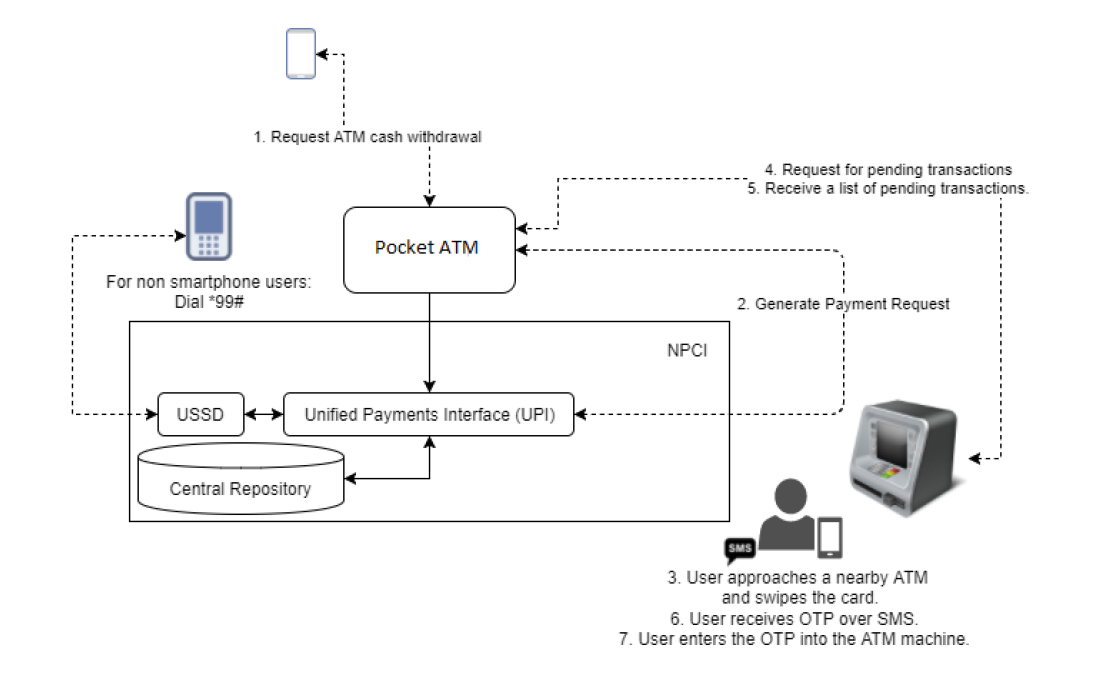
\includegraphics[width=250px]{pocketatmarchitecture}
    \caption{Cash Withdrawal workflow with PocketATM}
    \label{fig:pocketatm_architecture}
\end{figure}

\subsection*{Step 0: Registration \& Login into the system from phone}
\label{ssec:step0}

As a part of setup, the user logs in to their internet banking application on their smartphone. When the application starts up for the first time, it requests the user to set a 4-digit Mobile PIN (MPIN) for the device that the user is operating from. [In the backend the application then triggers an SMS with a cryptographic identity (public key) to the banking servers and maps the bank accounts registered to the mobile number with this identity.] Subsequently, after the registration of the device identity, when using the banking application from the same device the user can authenticate to access their banking account information with the MPIN that was previously set.

\subsection*{Step 1: Pre-authorize a transaction from phone}
\label{ssec:step1}

Once the user logs into the application successfully, they see a list of possible options and services that can be availed via the app. This includes a list like fund transfer, check account balance, transaction history etc.., [Here, the banking provider integrating PocketATM can add an option to Withdraw Cash from an ATM, as shown in the figure ~\ref{fig:UIProposals}.] On selecting this option, the user is presented a screen where they can pre-authorize the transaction. In this screen, the user can choose one of their accounts, to withdraw the cash, provided as a drop-down list. The user would then enter the amount that they would like to withdraw, and click/tap the pre-authorize button thereby pre-authorizing a transaction.

\begin{figure}
    % \centering
    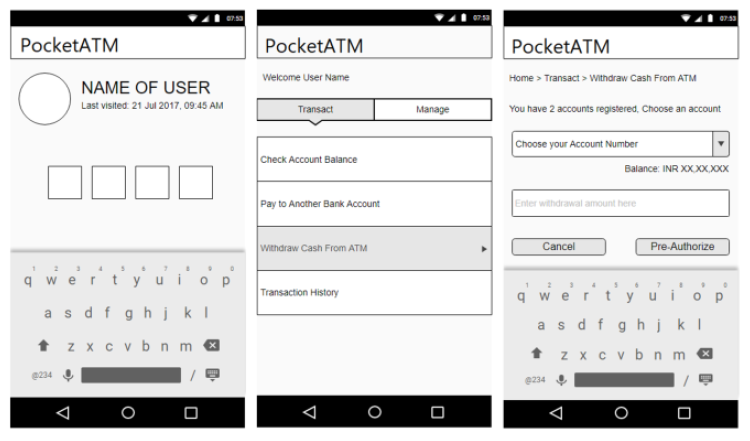
\includegraphics[width=250px]{pocketatmaccountpicker}
    \caption{Screenshots of the proposed updates to Internet Banking application}
    \label{fig:UIProposals}
    {\textit{(Left-Right: Login screen asking the user for the PIN, Addition of the cash withdrawal option, Account picker and pre-authorization screen to create a transaction request)}}
\end{figure}

\subsection*{Step 2: Authentication at the ATM \& Cash Withdrawal}
\label{ssec:step2}

After the transaction has been pre-authorized from the user's smartphone, they visit an ATM (even those that do not have accessible interfaces). First, the user swipes their ATM or debit card. The ATM screen shows the amount to be withdrawn and requests for the OTP. The user receives an OTP on their registered mobile number. They then enter this OTP into the machine. The machine verifies the OTP, authorizes the user and dispenses the cash.  

Alternatively, the user can also enter the OTP received, using the mobile application on the phone itself instead of on the ATM. To complete the transaction in this case the user would need to have cellular connectivity. Such a system would be useful in regions which have ATMs with inaccessible numeric keypads. 

The reason to choose OTP is primarily because, in India, OTP is already commonly used as a standard 2 factor authentication system for existing services, from ordering food online to financial transactions. Incoming messages to a mobile device do not incur any additional charges to the recipient, and hence using OTP as an authentication means seems practical.

In case the ATM has insufficient funds or has other technical difficulties, the user receives this information through SMS on their phone, in addition to the ATM's screen displaying the information regarding the issue. The user can read this error/information message using the screen reader on their mobile device.

\subsection{System Design}
\label{ssec:systemdesign}

Our proposed system builds on top of the Unified Payments Interface (UPI) platform that the Indian government has recently launched for making seamless inter-bank transactions~\cite{UPI}. While the UPI platform developed by IndiaStack forms the core, our proposal in this paper is to create a service layer for PocketATM, a central server in addition to the centralized infrastructure maintained by National Payments Corporation of India (NPCI)~\cite{NPCINUUP}, as shown in figure ~\ref{fig:pocketatm_architecture}. In PocketATM each ATM machine is treated as a special user and is provided a unique virtual payment address (VPA) which identifies the system on the network. The uniqueness of the addresses is guaranteed by the UPI platform. With this, each bank user and machine now have unique identifiers throughout the network. While the UPI system serves as a backbone to prototype PocketATM in India, a similar solution can be implemented using the national payment infrastructure of any other country, if it provides 1) the ability to uniquely identify users \& ATM machines, 2) have centralized management systems to monitor the ATMs and 3) enable easy and quick inter-bank payments.

\subsection*{Infrastructure Requirements for Implementation}
\label{ssec:infrastructurerequirements}

Every ATM in India is connected via the banking servers to a national financial network. PocketATM requires a backend software update to the infrastructure which grants each ATM a unique virtual payment address (VPA) like \textit{blratm1@PocketATM}. Using CMMS, the existing ATM infrastructure management system, the assignment of unique identities to each of these ATM machines can be implemented easily. The CMMS is already being used to monitor the status of the ATMs. All the ATMs are connected to NPCI and can make an additional request via the existing secure financial channel to the PocketATM service. 

\subsection*{Interacting with PocketATM Infrastructure Layers}
\label{ssec:interactionpocketATMInfra}

Since PocketATM is a re-design at the service layer, the functionality that this system offers can be integrated into the users' existing internet banking apps by a banking provider. For this reason, we will not have additional registration, login, etc., as the authentication mechanism would be handled by the respective banking application. Only a specific whitelist of banking servers would be able to register a pre-authorized request to the PocketATM service, to avoid any possibility of an attack from the client devices.

\subsection*{PocketATM: Under The Hood}
\label{ssec:underthehood}

The APIs exposed from the PocketATM services if leveraged by existing mobile banking applications facilitate pre-authorization requests to make a cash withdrawal. On successfully making a request to the PocketATM service, the service initiates a collect request leveraging the UPI platform. At this step, a collect request is raised to the user's bank account using the user's VPA and is maintained as a pending transaction. When the user reaches a nearby ATM and inserts their card into the card reader slot, the ATM picks up the user's pending transaction from PocketATM servers and sends a one-time password (OTP) to the registered mobile device. The user can then enter the OTP on the mobile application or use the physical ATM keypad to complete the pre-authorized transaction. 

The proposed system can also be extended to non-smartphone ATM users.

\subsection*{Extending PocketATM to non-smartphone users}
\label{ssec:extendingpocketatm}

The use of the Unified Payments Interface and a central server gives us the opportunity to expand the interaction in several ways.

\subsubsection*{\textbf{\textit{Using IVR Systems: }}}
\label{sssec:IVR}

We can introduce toll-free contact numbers, with an IVR (Interactive Voice Response) system enabling the users to interact and make pre-authorization ATM transactions via a phone call. This would enable those without smart phone access to use the new system as well. A user leveraging this feature would interact with the system as follows: 

\begin{enumerate}
    \item The user dials a toll-free number from their registered mobile devices.
    \item The IVR hangs up and then initiates a call to the mobile device.
    \item The IVR requests the user to authenticate themselves using their date of birth in DDMMYYYY format with a trailing \#
    \item The IVR on successful authentication asks the user to choose from a list of service options.
    \item Once the user chooses the number corresponding to the cash withdrawal option, the IVR requests the user to choose the account number from which the transaction needs to be made.
    \item After choosing the account number, the user is asked for the amount that they would wish to withdraw.
    \item A successful pre-authorization request has been placed and now the user can visit the ATM to withdraw the required amount.
\end{enumerate}

\subsubsection*{\textbf{\textit{Using USSD:}}}
\label{sssec:USSD}
In addition to using an IVR system, PocketATM also gives us the advantage of being able to use USSD (Unstructured Supplementary Service Data) to perform ATM transactions~\cite{perrier2015ussd}. 

The NPCI has developed NUUP (National Unified USSD Platform) on top of UPI platform and enables users without smartphones or internet access to perform most banking transactions~\cite{NPCINUUP}. This system has been launched by the government of India in 2014 and supports over 10 regional languages.

\subsubsection*{\textbf{\textit{Security Assumptions of PocketATM:}}}
\label{sssec:securityassumptions}

PocketATM piggy backs on the UPI infrastructure, which is currently deployed with all banks operating in India. An interface from this infrastructure is used for existing payment gateways like Google Pay (Tez)~\cite{GoogleTez}, Amazon Pay~\cite{AmazonPay}, PayTM~\cite{PayTM} and BHIM~\cite{BHIM}. Since PocketATM takes a similar approach, the system will be as secure as the existing UPI systems/payment gateways.

\section{Phase 3: Preliminary Evaluation of PocketATM}
\label{sec:phase3evaluation}

In this section we performed a preliminary usability study of the PocketATM system.

\subsection{Experimental Process}
\label{ssec:experimentalprocess}

The study was conducted with 19 participants from the same set of 22 participants during the Phase 2 interviews. Three participants had opted out of the study at the end of the second phase. To maintain consistency the same author (from Phase 2) acted as the experimenter for all the participants, while the other author made observations and took notes. Participants came in one at a time into the room where the mock PocketATM system was set up. Participants' consent was taken, making them aware of the study. The author briefly explained the scope of the study, explained how the system worked and told the participants the task that they would have to complete. The authors did not however, give the participants a sample task. In each case, we logged all interactions with the interface for later analysis. We tracked the number of errors on each screen; this included the number of backspaces entered while using the application.  Time taken for completion of the task was recorded. At the end of the last task, the author spoke with participants about their experience completing the tasks and listened to their feedback. Participants were then thanked and given a gift worth INR 500 (approx. 8 USD) for their participation.

\subsection{Technical Setup}
\label{ssec:technicalsetup}

The PocketATM prototype had 2 main user facing components. The first component was the PocketATM mock mobile application, where the user pre-authorized a transaction. The second, was the mock ATM that the user used to complete the cash withdrawal. 

The PocketATM mobile application was simulated as an existing Internet banking application. All of the transaction information was stored in a database. We tracked the time taken for the entire flow starting from login until a successful transaction. To ensure that we had data only for the interactions, the system was configured to stop the timer if there was no activity on the screen for 5 seconds. The timer was configured to resume immediately on any user activity or touch. This helped us to accurately measure only the active usage time of the prototype. 

The PocketATM infrastructure was setup to connect to the database of pre-authorized transactions that resulted from participants' interactions with the internet banking mock application. An OTP based authentication procedure was used to grant access to a user's pre-approved transactions. 

The ATM was mocked up as a web application in the experiments. We set up a laptop with a screen reader installed. This laptop was running the mock PocketATM application. The web application was configured to automatically set screen reader focus on to fields that required user input, without the user having to navigate by pressing tab, shift+tab, etc. This was done to ensure behavior similar to a real ATM where the user would not have access to these options. Moreover, the mock ATM (the laptop) had a keyboard with just the number pad exposed attached. The keys were reprogrammed to be in the same order as the numeric keypad on the ATM machine. This served as analogous to the keypad on traditional ATMs.

\subsection{Task}
\label{ssec:task}

Participants were required to use the PocketATM system to withdraw INR 500 (approx. 8 USD) from their mock accounts. This required the following steps:

\subsubsection*{\textit{\textbf{Stage 1: Pre-authorization from the smartphone.}}}

The participants were asked to open the mobile application on their smartphone and follow the on-screen instructions. The application consisted of a login page where the user entered their phone number after which the users were taken to a page that allowed them to choose their account from a list of preset accounts. Then enter 500 INR (approx. 8 USD) as the amount they wish to withdraw and pre-authorize the transaction after reviewing it. This would then create a transaction record in the PocketATM database.

\subsubsection*{\textit{\textbf{Stage 2: Interacting with the PocketATM Prototype.}}}

The interface on the ATM first required the users to simulate a card being inserted into a slot like that of a real ATM. To facilitate this, we placed a cardboard prop containing a slot similar to that of a real ATM and gave the users a non-functional ATM card. The participant would enter their phone number onto the ATM, which then sent the OTP to their mobile phone. (In a real world PocketATM system, the users would not have to enter their phone number since this information would be linked to their card and could be retrieved by the service after the card was inserted.) The user then entered the OTP and completed the transaction that was pre-authorized.

\section{Results}
\label{sec:results}

As our main interest is how the system was used, we focus primarily on the time taken for completion of transactions, errors made, and feedback from participants on the PocketATM system. 

We observed improvements in time taken to successfully perform a transaction on PocketATM. For a VIP to perform a complete transaction on existing accessible ATMs, the average time taken is roughly 4 minutes (as per our surveys and interviews conducted earlier). PocketATM with 26 ATM transactions (Each participant completed at least one transaction, 4 participants completed multiple transactions) shows an average of 59.84 seconds to withdraw the required cash (this excludes the time taken for pre-authorization on the smartphone).  

The average time required to use the smartphone application for making a successful pre-authorization request was 109.41 seconds. A total of 58 pre-authorized transactions were sent to the server by the participants (Each participant made at least two pre-authorization requests from the mobile app while some of them made more than two requests). We observed that the time taken can reduce with practice over time. The data in the table ~\ref{tab:preauth} is for three of the 19 participants, who used the mobile application three separate times each to pre-authorize the transactions.

% Please add the following required packages to your document preamble:
% \usepackage{multirow}
\begin{table}[h]
\begin{tabular}{|l|l|l|l|}
\hline
\multirow{2}{*}{Participant \#} & \multicolumn{3}{l|}{\begin{tabular}[c]{@{}l@{}}Time Taken to Register a transaction \\ from the mobile application (seconds)\end{tabular}} \\ \cline{2-4} 
 & Attempt 1 & Attempt 2 & Attempt 3 \\ \hline
P10 & 184.25 & 105.63 & 67.35 \\ \hline
P14 & 170.21 & 109.14 & 79.24 \\ \hline
P15 & 169.23 & 138.73 & 78.96 \\ \hline
\end{tabular}
\caption{Time taken to create a pre-authorized transaction}
\label{tab:preauth}
\end{table}

We observed that the maximum number of errors were made when pressing the login button on the 1st screen of the mobile application. This error happened with 12 participants. Participants with low vision reported that they could not see the login button because the text box for the phone number took up most of the screen space, when a screen magnifier was used. Participants using screen readers expected the system to login after entering the 10th digit into the phone number field, like a regular pass code, without explicitly clicking on the login button. This was more common in VIPs with lesser experience using technology applications.  VIPs with higher technological proficiency who knew about forms, expected a submit button to complete the required action. 

During PocketATM's usage, 4 errors were recorded while sending the OTP via SMS to the participants in the total of the 26 transactions. The participants never received the OTP in these 4 instances because they were registered on their carriers' Do Not Disturb (DND), service which blocked out the SMS provider that we were using. This problem however would not happen in a real world implementation of banks' SMS gateway since banking providers are whitelisted by the carriers. 

\subsection{Feedback from Participants}
\label{ssec:feedback}

After the usability test, participants provided feedback on their experiences using PocketATM.

\subsubsection*{\textit{\textbf{Concerns with Delivery of OTP while using PocketATM:}}}
\label{sssec:otpdelivery}

Most of these concerns were with respect to the longevity of the OTP pin, incorrectly entered OTP and consequences if an OTP is not received on the phone when one is at the ATM trying to complete a pre-authorized transaction.

\textcolor{quotegray}{\say{\textit{Is there something I can do when I do not receive an OTP to my phone? If I enter a wrong OTP into the ATM, what will happen? When will I get a new OTP?}} -P3}

Not receiving an OTP on the phone would prevent the user from using the ATM. In our study the error occurred because of an external SMS provider we used. In a real world implementation there could be outages in the network which might delay the OTP. 

On entering a wrong OTP into the ATM, the system would ask the user to reenter thus giving them one more chance. On failing to enter correctly for the second time, the ATM would return the inserted card and abort the transaction. Re-inserting the card into the ATM would provide a new OTP to the user. After failing to enter the correct password in a fixed number of attempts (three in most cases), the card of the account holder would get temporarily locked~\cite{SBITOS}.

\subsubsection*{\textit{\textbf{Ease of Usage of PocketATM:}}}
\label{sssec:easeofusage}

Participants reported that they found the system easy to use.

\textcolor{quotegray}{\say{\textit{I really like this system, insert a card, get the OTP and carry the money. I do not even need to carry a headset and look for a headphone slot on the ATM machine. I really like this.}} -P6}

\textcolor{quotegray}{\say{\textit{Operating everything on the phone and the ATM card being the entire connector to the puzzle is really nice. It'll be extremely useful to VIPs like me}} -P2}

For overall experience, participants rated PocketATM an average of 9.1 on a 10 point likert scale. Some participants mentioned that they take help from their family or friends to visit ATMs for transactions, but with a system like PocketATM they could be more independent. 

\subsubsection*{\textit{\textbf{Suggestions:}}}
\label{sssec:suggestions}

Our implementation was a little confusing for the users with low vision, because of the login button. In the future we aim to overcome this issue by making the application interfaces more adaptive to users who use screen magnifiers.

\textcolor{quotegray}{\say{\textit{I know that the application was currently built keeping completely blind users in mind. For someone like me with low visibility, I could not find the login button, so I activated my screen reader instead and used the application and found the login button.}} -P2}

Participants wanted the PocketATM system to help identify the type of currency notes that the ATM would dispense. In 2016, the government of India announced the demonetisation of all INR 500 and INR 1000 banknotes to help curtail the shadow economy and crack down on the use of illicit and counterfeit cash. The new INR 500 and INR 1000 have a  different size and feel compared to the previous notes and have been reported to not be accessible to VIPs~\cite{HTArticle}.

\textcolor{quotegray}{\say{\textit{I really like this system but I wish there was more information that was given to me like the denomination of the notes I received. I currently use another app to scan the notes and find its denomination. It'd be nice if this information was also provided in an SMS after the transaction so that I can organize my wallet.}} -P3}

\section{Conclusion \& Future Work}
\label{sec:conclusion}

A decade since the Indian central government authority's mandate to make ATMs accessible, the number of accessible ATMs still remains less than the suggested 33\%. Moreover, the physical variations in these machines make it quite difficult for a VIP to quickly find the headphone jack and enable voice guidance in the first place. This gap can be attributed to a lack of emphasis on accessible design and a weak policy suggesting that an accessible ATM merely speak (Most ATMs hard-code static messages just saying \textit{`Hello'} \& \textit{`Thank you'} meeting the policy requirements but these are not really useful). An immediate possible outcome from the survey is a map that would help a VIP wanting to make an ATM transaction locate the nearest accessible ATM. More crowd sourcing can be done to add information such as the location of the headphone jack, availability of braille labels and wheel chair accessibility. 

The context for our effort is set in India, but we believe that our approach towards ATM accessibility could be adapted, with appropriate modifications, by other countries with similar financial infrastructures. That said, validating this assumption would require more in-depth exploration in other developing countries and the authors believe that it would be a worthwhile study that could be done in the near future. Moving forward, we plan to collaborate with NPCI and pilot the PocketATM system to further evaluate its usability over a long term. The need for accessibility to perform financial transactions independently opens up new opportunities to explore accessible and usable interfaces to make these transactions. 

It would be interesting to do a comparative study between the usability of existing ATMs and the PocketATM system with VIPs. 

PocketATM also opens up opportunities to understand accessibility implications for people with mobility impairments.
 

%\end{document}  % This is where a 'short' article might terminate
\section*{Appendix}
\appendix

\section{Survey Questions}
\label{appendix:surveyquestions}

\begin{enumerate}
    \item On a scale of 1-10 please rate your experience with the ATM machine.
    \item What do you think about the cash withdrawal experience?
    \item Do the systems' capabilities meet your requirements?
    \item Were the instructions and information given by the system effective/useful?
    \item Were the sequence of actions and items hard to remember?
    \item Was this a frustrating experience?
\end{enumerate}

\section{Phase 2 Demographic Survey Questions}
\label{appendix:phase2demographicsurveyquestions}

\begin{enumerate}
    \item What is your age group?
    \item What is your gender?
    \item Which of the following describes the nature of your visual impairment?
    \item Do you have an ATM debit/credit card?
    \item Have you used these cards in an ATM with sighted assistance?
    \item Have you used these cards in an ATM by yourself?
    \item Did you use a talking / accessible ATM?
    \item How often do you use an ATM?
    \item If you use a smartphone which smartphone do you use?
    \item Since how long have you been using a smartphone?
    \item Do you use a screen reader on your smartphone?
    \item Do you use internet/mobile banking apps like iMobile / SBI  Buddy / HDFC Bank etc.?
    \item What is the highest level of education you have received?
    \item Which of the following best describes your household expenditure?
    \item What are the difficulties you face with using the current ATM system?
\end{enumerate}


\section{Survey Questions Used in Field Study}
\label{appendix:fieldsurveyquestions}

\begin{enumerate}
    \item Can you share the map location of the ATM?
    \item Which bank does this ATM belong to?
    \item Which of the headphone jacks did the ATM machine have?
    \item Did the ATM provide you with an option to enable voice guidance?
    \item Did the ATM machine give an option to turn off the screen?
    \item Did the ATM announce \textit{hello} and \textit{thank you} messages?
    \item Did the ATM announce options such as \textit{"balance enquiry"}, \textit{"check balance"}, \textit{"get statement"}?
    \item Which features of the ATM did you use with the help of voice feedback?
    \item How long did you take to use the ATM services with voice guidance?
\end{enumerate}

\begin{acks}
The authors would like to thank Mr. Moses Chowdary from Enable India~\footnote{http://www.enableindia.org/} and Sri Mahantesh, Mr. Muralidhara from Samarthanam Trust~\footnote{http://www.samarthanam.org/} for their assistance during the preliminary studies and testing of PocketATM. The authors would also like to thank Mr. Rakesh Dubbudu from Factly\footnote{https://factly.in/} for feedback and advice while filing an RTI request. The authors would also like to thank Dr. William Thies \& Dr. Manohar Swaminathan from Microsoft Research India for their valuable feedback during this effort.
\end{acks}


\bibliographystyle{ACM-Reference-Format}
\bibliography{bib}

\end{document}
